\documentclass[11pt,a4paper]{article}
\usepackage[T1]{fontenc}
\usepackage[utf8]{inputenc}
\usepackage{lmodern}
\usepackage[margin=2.4cm]{geometry}
\usepackage{amsmath,amssymb}
\usepackage{booktabs,tabularx}
\usepackage{graphicx}
\usepackage{xcolor}
\usepackage{listings}
\usepackage{enumitem}
\usepackage[colorlinks=true,linkcolor=blue!50!black,urlcolor=blue!50!black]{hyperref}

\definecolor{shellbg}{gray}{0.95}
\lstset{basicstyle=\ttfamily\small, backgroundcolor=\color{shellbg}, frame=single,
  rulecolor=\color{gray!60}, breaklines=true, columns=fullflexible, keepspaces=true,
  showstringspaces=false, xleftmargin=2pt, xrightmargin=2pt, aboveskip=6pt, belowskip=6pt,
  literate={~}{{\textasciitilde}}1}
\newcommand{\f}[1]{\texttt{#1}}
\setlist{itemsep=2pt,topsep=4pt}
\setlength{\parindent}{0pt}
\setlength{\parskip}{5pt}
\sloppy

\title{ALF output in pandas:\\ the \texttt{alf\_to\_pandas.py} tables}
\author{Companion to \texttt{ALF\_SZ\_Manual.pdf}}
\date{November 2026}

\begin{document}
\maketitle
\tableofcontents

%=======================================================================================
\section{What ALF writes, and why there are so many files}
%=======================================================================================

ALF stores \emph{every bin}. A bin is the average over \f{NSweep} sweeps; one line (or one
block) per bin is appended to the raw files while the simulation runs. The analysis program
\f{ana.out} turns these bins into means with jackknife error bars. A run directory therefore
contains two kinds of files for each observable \f{X}:

\begin{center}
\small
\begin{tabularx}{\textwidth}{>{\raggedright\arraybackslash}p{3.6cm}l>{\raggedright\arraybackslash}X>{\raggedright\arraybackslash}p{2.3cm}}
\toprule
file & written by & content & DataFrame \\
\midrule
\f{X\_scal}  & \f{ALF.out} & raw bins of a scalar observable & \f{scal\_bins} \\
\f{X\_eq}    & \f{ALF.out} & raw bins of an equal-time correlation, in $\mathbf k$-space & \f{eq\_bins}, \newline \f{eq\_back} \\
\f{X\_tau}   & \f{ALF.out} & raw bins of a time-displaced correlation & \f{tau\_bins} (optional) \\
\midrule
\f{X\_scalJ} & \f{ana.out} & mean $\pm$ error (and average sign) & \f{scal} \\
\f{X\_eqJK}  & \f{ana.out} & $C(\mathbf q)$ $\pm$ error & \f{eq} \\
\f{X\_eqJR}  & \f{ana.out} & $C(\mathbf r)$ $\pm$ error & \f{eq\_r} \\
\f{X\_<kx>\_<ky>/g\_dat}, \newline \f{X\_R0/g\_dat} & \f{ana.out} & $C(\mathbf q,\tau)$ and $C(\mathbf r{=}0,\tau)$ $\pm$ error & \f{tau} \\
\f{X\_tauJK} & \f{ana.out} & susceptibility $\chi(\mathbf q)=\int_0^\beta d\tau\, C(\mathbf q,\tau)$ & \f{chi} \\
\midrule
\f{parameters} & you & input namelists & \f{params} \\
\f{info}     & \f{ALF.out} & acceptance, numerical precision, CPU time & \f{info} \\
\f{X\_*\_info} & \f{ALF.out} & lattice description (not read) & -- \\
\f{confout\_*}, \f{seeds} & & last configuration, random seeds (not read) & -- \\
\bottomrule
\end{tabularx}
\end{center}

\textbf{For results you normally only need the \f{ana.out} tables} (\f{scal}, \f{eq},
\f{eq\_r}, \f{tau}, \f{chi}). The raw bins are for checking thermalisation and for error bars of
quantities that ALF does not compute itself (Sec.~\ref{sec:jackknife}).

\paragraph{Reading the numbers by hand.}
ALF writes Fortran notation with the mantissa between 0.1 and 1:
\f{-0.56572447387401041E+001} $=-0.5657\times10^{1}=-5.657$. The script converts everything to
ordinary floats.

\paragraph{Sign-weighted bins.}
A raw bin does not contain $\langle O\rangle$ but $\langle O\,s\rangle_\text{bin}$ and
$\langle s\rangle_\text{bin}$, with $s$ the sign (phase) of the Monte Carlo weight. The
estimate is $\langle O\rangle=\sum_\text{bins}\langle Os\rangle/\sum_\text{bins}\langle s\rangle$.
For your models $s=1$, so $\langle O s\rangle=\langle O\rangle$, but the script keeps both
columns so that it also works with a sign problem.

\paragraph{ALF appends.}
\f{ALF.out} appends new bins to existing files. A directory that has been used for two
different parameter sets contains a mixture of both. Use one directory per parameter set
(and continue runs only with unchanged parameters).

%=======================================================================================
\section{Using the script}
%=======================================================================================

The script is \f{ALF/Infos\_SZ/alf\_to\_pandas.py}. It needs \f{numpy} and \f{pandas}, works for
every ALF Hamiltonian (standard Hubbard, \f{Hubbard\_Sz}, \f{TwoBand\_Spin}, \dots) and reads
the text output (ALF built without \f{HDF5}). Run \f{ana.out} first (\f{run.sh} does it).

\subsection{In Python / Jupyter}
\begin{lstlisting}[language=Python]
import sys
sys.path.insert(0, "/Users/sbl848/Documents/ALF_QMC_PROJECT/ALF_SZ/ALF/Infos_SZ")
import alf_to_pandas as ap

d = ap.load_run("/Users/sbl848/Documents/ALF_QMC_PROJECT/QMC_Check")
print(d)                 # overview of all tables
d.scal                   # pandas DataFrame
\end{lstlisting}
\f{print(d)} lists all tables with their size and columns:
\begin{lstlisting}[basicstyle=\ttfamily\scriptsize]
ALFData with tables (rows x columns):
  params            1 x 55   run, path, ham_name, l1, l2, lattice_type, ..., n_skip, n_rebin, ...
  info              1 x 9    run, n_alf_calls, precision_green_mean, ..., acceptance, cpu_time_s
  scal              4 x 10   run, obs, comp, label, mean, error, sign, sign_error, n_bins, n_bins_eff
  scal_bins        80 x 9    run, obs, comp, label, bin, Os_re, Os_im, sign, value
  eq               20 x 10   run, obs, kx, ky, o1, o2, re, re_error, im, im_error
  eq_r             20 x 10   run, obs, rx, ry, o1, o2, re, re_error, im, im_error
  eq_bins         400 x 10   run, obs, bin, kx, ky, o1, o2, Os_re, Os_im, sign
  eq_back         100 x 7    run, obs, bin, orb, Os_re, Os_im, sign
  tau            3025 x 9    run, obs, kx, ky, tau, value, error, channel, point
  chi              20 x 8    run, obs, kx, ky, re, re_error, im, im_error
  tau_bins          -
\end{lstlisting}
Options of \f{load\_run(path, raw=True, raw\_tau=False, name=None)}:
\f{raw=False} skips the raw bins (faster for large lattices); \f{raw\_tau=True} also reads the
raw time-displaced bins, which can be large; \f{name} sets the value of the \f{run} column
(default: the directory name).

\subsection{Several runs}
\begin{lstlisting}[language=Python]
D = ap.load_runs(["~/QMC_runs/Heis_dt0.05", "~/QMC_runs/Heis_dt0.025"])  # a list ...
D = ap.load_runs("~/QMC_runs/Heis_*")                                      # ... or a glob pattern
\end{lstlisting}
All tables of all runs are stacked; the column \f{run} tells them apart, and \f{D.params} has
one row per run. To attach parameters to results, merge on \f{run} (example in
Sec.~\ref{sec:examples}).

\subsection{Command line and saving}
\begin{lstlisting}
python3 alf_to_pandas.py RUN_DIR [RUN_DIR ...]              # overview + scalar results
python3 alf_to_pandas.py ~/QMC_runs/Heis_* --pickle all.pkl # save all tables
python3 alf_to_pandas.py ~/QMC_runs/Heis_* --csv tables/    # one CSV file per table
\end{lstlisting}
In Python: \f{d.to\_pickle("all.pkl")}, \f{d.to\_csv("tables/")}. Load the pickle with
\f{tables = pandas.read\_pickle("all.pkl")}, a dictionary \f{\{"scal": DataFrame, ...\}}.

%=======================================================================================
\section{The tables}
%=======================================================================================

Common columns: \f{run} (run name), \f{obs} (observable = file name prefix, e.g.\ \f{Ener},
\f{SpinZ}). Momenta \f{kx}, \f{ky} are in radians, exactly as ALF lists them (on $2\times2$: $0$ and
$\pi$); compare them with \f{np.isclose}. Orbital indices \f{o1}, \f{o2} start at 1.

\subsection{\texttt{params} and \texttt{info} (one row per run)}
\f{params}: \f{run}, \f{path}, and every parameter of the namelists that ALF used for this
model (\f{VAR\_ham\_name}, \f{VAR\_lattice}, \f{VAR\_Model\_Generic}, \f{VAR\_<ham\_name>},
\f{VAR\_QMC}, \f{VAR\_errors}). Names are \emph{lower case}: \f{ham\_u}, \f{beta}, \f{dtau},
\f{l1}, \f{n\_skip}, \f{ham\_int}, \dots\ The namelists of other models in the same file are
ignored (the standard parameter file contains e.g.\ \f{Beta} in several of them).

\f{info}: \f{n\_alf\_calls} (how often \f{ALF.out} ran in this directory; $>1$ for continued
runs), \f{precision\_green\_mean/max}, \f{precision\_phase\_max},
\f{precision\_tau\_mean/max}, \f{acceptance}, \f{cpu\_time\_s} (of the last call).

\subsection{\texttt{scal}: scalar results (\texttt{X\_scalJ})}
\begin{center}\small
\begin{tabularx}{\textwidth}{lX}
\toprule
column & meaning \\
\midrule
\f{obs}, \f{comp}, \f{label} & observable, component (1, 2, \dots), readable name: \f{Ener}, \f{Kin}, \f{Pot}, \f{Part}; for \f{Part\_cd} the components are labelled \f{N\_c}, \f{N\_d} \\
\f{mean}, \f{error} & jackknife mean and error \\
\f{sign}, \f{sign\_error} & average sign \\
\f{n\_bins}, \f{n\_bins\_eff} & bins in the file; bins used after \f{n\_skip} and \f{N\_rebin} \\
\bottomrule
\end{tabularx}\end{center}
Quantities are totals over the lattice (divide by $L_1L_2$ for per-site values).

\subsection{\texttt{scal\_bins}: raw bins of scalars (\texttt{X\_scal})}
\f{obs}, \f{comp}, \f{label} as above; \f{bin} (1, 2, \dots, including the thermalisation
bins); \f{Os\_re}, \f{Os\_im} $=\langle O s\rangle_\text{bin}$; \f{sign} $=\langle s\rangle_\text{bin}$;
\f{value} $=$ \f{Os\_re}/\f{sign}, the bin average of $O$. Use \f{value} to look at bins, and
\f{Os\_re}, \f{sign} for the jackknife.

\subsection{\texttt{eq}: equal-time correlations in momentum space (\texttt{X\_eqJK})}
For each $\mathbf q=$ (\f{kx}, \f{ky}) and orbital pair (\f{o1}, \f{o2}):
\begin{equation}
  C_{o_1o_2}(\mathbf q)=\frac1N\sum_{i,j}e^{i\mathbf q\cdot(\mathbf r_i-\mathbf r_j)}
  \Bigl(\langle O_{i,o_1}O_{j,o_2}\rangle-\langle O_{o_1}\rangle\langle O_{o_2}\rangle\Bigr),
\end{equation}
columns \f{re}, \f{re\_error}, \f{im}, \f{im\_error}. The background
$\langle O\rangle\langle O\rangle$ only contributes at $\mathbf q=0$. Examples: \f{SpinZ} at
$(\pi,\pi)$ is the antiferromagnetic structure factor $S^{zz}(\pi,\pi)$; \f{Pair} at $\mathbf
q=0$ is the pair structure factor.

\textbf{Orbitals.} \f{SpinX/Y/Z}, \f{Pair}, \f{SpinT}, \f{SpinXY} have one orbital
(\f{o1} = \f{o2} = 1). \f{Green} and \f{Den} are orbital resolved; the script adds columns
\f{o1\_name}, \f{o2\_name}: \f{c}, \f{d} for \f{Hubbard\_Sz}; \f{c\_up}, \f{c\_dn}, \f{d\_up},
\f{d\_dn} for \f{TwoBand\_Spin}. (For other models the names are the indices.)

\subsection{\texttt{eq\_r}: equal-time correlations in real space (\texttt{X\_eqJR})}
Same as \f{eq} with \f{rx}, \f{ry} $=\mathbf r$ instead of $\mathbf q$:
$C_{o_1o_2}(\mathbf r)=\frac1N\sum_i\bigl(\langle O_{i+\mathbf r,o_1}O_{i,o_2}\rangle-\langle O\rangle\langle O\rangle\bigr)$,
and $C(\mathbf q)=\sum_{\mathbf r}e^{i\mathbf q\cdot\mathbf r}C(\mathbf r)$.
Example (Hubbard, $S^z_i=n_{i\uparrow}-n_{i\downarrow}$): \f{SpinZ} at $\mathbf r=0$ is
$\langle(S^z_i)^2\rangle=1-2\langle n_\uparrow n_\downarrow\rangle$.

\subsection{\texttt{eq\_bins}, \texttt{eq\_back}: raw bins of equal-time correlations (\texttt{X\_eq})}
\f{eq\_bins}: \f{bin}, \f{kx}, \f{ky}, \f{o1}, \f{o2}, \f{Os\_re}, \f{Os\_im}, \f{sign}; the
$\mathbf q$-space correlation of one bin, \emph{without} background subtraction.
\f{eq\_back}: \f{bin}, \f{orb}, \f{Os\_re}, \f{Os\_im}, \f{sign}; the background
$\langle O_\text{orb}\rangle$ of each bin. A jackknife of \f{eq\_bins} reproduces \f{eq} at
every $\mathbf q\neq0$; at $\mathbf q=0$ it agrees only if $\langle O\rangle=0$ (e.g.\ not for
\f{Den}). For $\mathbf q=0$ use \f{eq}.

\subsection{\texttt{tau}: time-displaced correlations (\texttt{g\_dat} files of \texttt{ana.out})}
\f{kx}, \f{ky}, \f{tau}, \f{value}, \f{error}, \f{channel}, \f{point}. One row per $\mathbf q$
and $\tau$, from the directories \f{X\_<kx>\_<ky>/g\_dat} (\f{point} = \f{"k"}) and
\f{X\_R0/g\_dat} (\f{point} = \f{"R0"}, local correlation, \f{kx} = \f{ky} = NaN).
Only with \f{Ltau = 1}. Notes:
\begin{itemize}
  \item \f{value} is summed over the orbitals of the unit cell (ALF writes no orbital-resolved
        $C(\mathbf q,\tau)$ here). For one-orbital observables this is $C(\mathbf q,\tau)$ itself.
  \item The momenta come from the directory names, which \f{ana.out} writes with two decimals
        and as absolute values: $\pi$ appears as \f{3.14}. Select them with
        \f{np.isclose(kx, 3.14)} or \f{kx > 3}.
  \item \f{channel} \f{PH} (density, spin) and \f{PP} (pairing): \f{ana.out} uses
        $C(\tau)=C(\beta-\tau)$ and writes $0\le\tau\le\beta/2$. Channel \f{P} (\f{Green}):
        $0\le\tau\le\beta$.
\end{itemize}

\subsection{\texttt{chi}: susceptibilities (\texttt{X\_tauJK})}
\f{kx}, \f{ky}, \f{re}, \f{re\_error}, \f{im}, \f{im\_error}:
$\chi(\mathbf q)=\int_0^\beta d\tau\sum_{o_1o_2}C_{o_1o_2}(\mathbf q,\tau)$ (trapezoidal rule,
background subtracted at $\mathbf q=0$). Example: \f{SpinZ} at $(\pi,\pi)$ is the staggered
spin susceptibility.

\subsection{\texttt{tau\_bins}: raw time-displaced bins (\texttt{X\_tau}, optional)}
As \f{eq\_bins} with an additional column \f{tau}. Read only with \f{raw\_tau=True}; size
$=N_\text{bins}\times N\times(\beta/\Delta\tau+1)\times N_\text{orb}^2$ rows per observable.

%=======================================================================================
\section{Error bars of derived quantities: \texttt{jackknife}}
\label{sec:jackknife}
%=======================================================================================

Error bars of a function of averages (a ratio, a per-site value with a parameter, a
difference of two observables) cannot be obtained from \f{mean} and \f{error} alone, because
the observables are correlated. The jackknife over bins handles this:
\begin{lstlisting}[language=Python]
mean, err = ap.jackknife(Os, sign, func=None, n_skip=0, n_rebin=1)
\end{lstlisting}
\f{Os}: array of \f{Os\_re} per bin, shape (bins,) or (bins, $m$) for $m$ observables;
\f{sign}: \f{sign} per bin; \f{func}: function of the $m$ averaged observables (default:
identity); \f{n\_skip}, \f{n\_rebin} as in the parameter file. The convention is that of
\f{ana.out}: $\sigma^2=N\cdot\mathrm{Var}_\text{jk}$ with $N$ the number of (rebinned) bins.
(The textbook jackknife uses $N-1$; the difference is a factor $\sqrt{N/(N-1)}$.)

\f{ap.jackknife\_bins(table, n\_skip, n\_rebin)} applies the jackknife to every group of a
raw-bin table and returns \f{mean}, \f{error}. Applied to \f{scal\_bins} with the run's
\f{n\_skip} and \f{n\_rebin}, it reproduces \f{scal} to machine precision.

%=======================================================================================
\section{Examples}
\label{sec:examples}
%=======================================================================================
All examples below were run on the $2\times2$ Hubbard run in \f{QMC\_Check} ($U=4$,
$\beta=20$) and on the Heisenberg $\Delta\tau$ series of the manual. Start with
\begin{lstlisting}[language=Python]
import numpy as np, pandas as pd, matplotlib.pyplot as plt
import alf_to_pandas as ap
d = ap.load_run("/Users/sbl848/Documents/ALF_QMC_PROJECT/QMC_Check")
\end{lstlisting}

\textbf{Energy.}\par
\begin{lstlisting}[language=Python]
E = d.scal.set_index("label").loc["Ener"]
print(f"E = {E['mean']:.4f} +- {E['error']:.4f}")       # E = -5.6572 +- 0.0089
\end{lstlisting}

\textbf{Structure factor at $(\pi,\pi)$.}\par
\begin{lstlisting}[language=Python]
Szz  = d.eq.query("obs == 'SpinZ'")[["kx", "ky", "re", "re_error"]]
pipi = Szz[np.isclose(Szz.kx, np.pi) & np.isclose(Szz.ky, np.pi)]   # 1.9214(59)
\end{lstlisting}

\textbf{Thermalisation and $C(\mathbf q,\tau)$} (Fig.~\ref{fig:ex}).\par
\begin{lstlisting}[language=Python]
fig, ax = plt.subplots(1, 2, figsize=(9, 3.2))
b = d.scal_bins.query("label == 'Ener'")
ax[0].plot(b["bin"], b["value"], "o-", ms=3)
ax[0].axvspan(0.5, d.params["n_skip"].iloc[0] + 0.5, color="0.85")  # discarded

c = d.tau.query("obs == 'SpinZ' and point == 'k' and (kx > 0 or ky > 0)")
for (kx, ky), g in c.groupby(["kx", "ky"]):
    ax[1].errorbar(g["tau"], g["value"], g["error"], fmt="o-", ms=2,
                   label=f"q = ({kx}, {ky})")
ax[1].legend()
\end{lstlisting}

\begin{figure}[h]
  \centering
  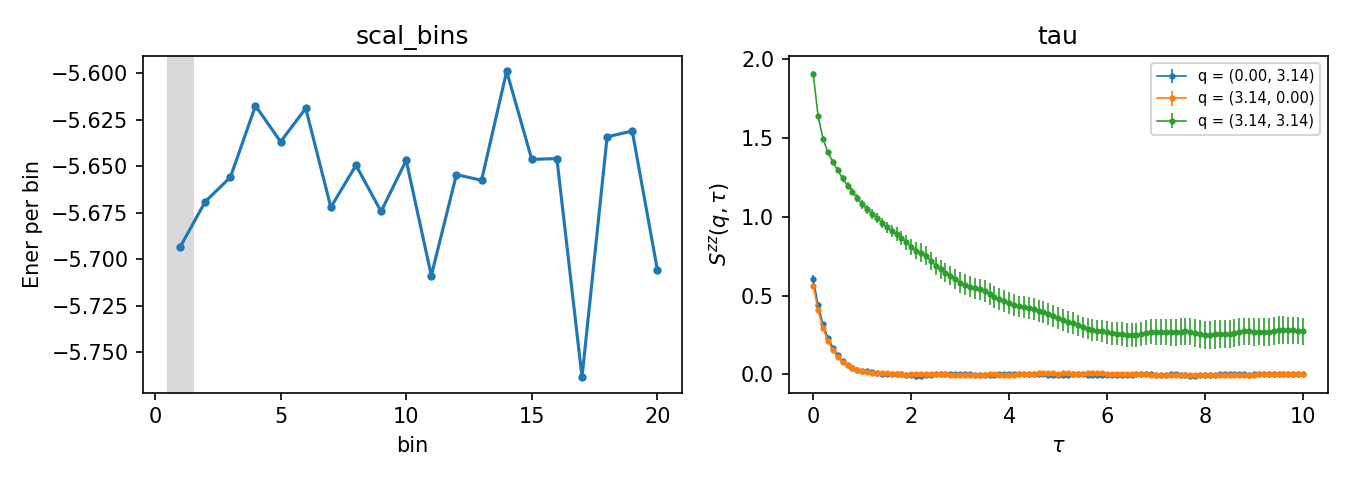
\includegraphics[width=\textwidth]{figures/pandas_example.png}
  \caption{Left: \f{Ener} per bin from \f{scal\_bins}; the grey bin is discarded
  (\f{n\_skip} $=1$). Right: $S^{zz}(\mathbf q,\tau)$ from \f{tau}, for $0\le\tau\le\beta/2$
  (channel PH). The slow decay at $(\pi,\pi)$ reflects the small spin gap of the $2\times2$
  cluster.}
  \label{fig:ex}
\end{figure}

\paragraph{Derived quantities with error bars.}
Double occupancy per site, $\langle n_\uparrow n_\downarrow\rangle=\text{\f{Pot}}/(UN)$, and the
ratio \f{Pot}/\f{Kin}:
\begin{lstlisting}[language=Python]
p = d.params.iloc[0]
N = p["l1"] * p["l2"]
b = d.scal_bins.query("label == 'Pot'").sort_values("bin")
docc = ap.jackknife(b["Os_re"], b["sign"], func=lambda O: O / (p["ham_u"] * N),
                    n_skip=int(p["n_skip"]))                     # (0.11652, 0.00065)

B = d.scal_bins.pivot_table(index="bin", columns="label", values=["Os_re", "sign"])
Os, sgn = B["Os_re"][["Pot", "Kin"]].to_numpy(), B["sign"]["Kin"].to_numpy()
ratio = ap.jackknife(Os, sgn, func=lambda O: O[0] / O[1], n_skip=int(p["n_skip"]))
# ratio = (-0.2479, 0.0013)
\end{lstlisting}

\textbf{Several runs: $\Delta\tau\to0$.}\par
\begin{lstlisting}[language=Python]
D = ap.load_runs("~/QMC_runs/Heis_test_2x2*")
kin = (D.scal.query("label == 'Kin'")
         .merge(D.params[["run", "dtau", "ham_int"]], on="run")
         .sort_values("dtau"))
fit = np.polyfit(kin["dtau"]**2, kin["mean"], 1, w=1/kin["error"])
print("Kin(dtau -> 0) =", fit[1])      # -13.540  (ED: -13.537)
\end{lstlisting}
The same pattern (\f{query} for the observable, \f{merge} with \f{params}) gives e.g.\
\f{Ener} against \f{ham\_u}, or $S(\pi,\pi)$ against \f{l1} for a finite-size scaling.

%=======================================================================================
\section{Checks and limitations}
%=======================================================================================
\begin{itemize}
  \item Tested on the standard Hubbard model, \f{Hubbard\_Sz} and \f{TwoBand\_Spin}
        (Ising, Heisenberg). The jackknife of the raw bins reproduces \f{ana.out} to
        $\sim10^{-15}$ for all scalars, for all equal-time correlations at $\mathbf q\neq0$, and
        for $C(\mathbf q,\tau=0)$.
  \item Text output only; ALF built with \f{HDF5} writes \f{data.h5} instead (not supported).
  \item Not read: \f{X\_*\_info}, \f{confout\_*}, covariance matrices in \f{g\_dat}
        (\f{N\_Cov = 1}).
  \item \f{jackknife} uses the real parts (\f{Os\_re}); imaginary parts vanish for sign-free
        real observables.
\end{itemize}

\end{document}
